\chapter{Desenvolvimento do Trabalho}\label{chap:atividadesRealizadas}

% Este capítulo não deve ultrapassar o total de 4 páginas.

\section{Atividades Realizadas}

Nas primeiras semanas de trabalho foi dada uma tarefa de implementação de um \gls{scheduler}, com uma interface para agendamento de scripts, como mostrada na Figura~\ref{fig:scheduler}. O \gls{scheduler} foi criado para funcionar dentro de um \gls{container} \gls{Docker}, no qual é possível controlar o estado de outros \glspl{container} sendo executados no mesmo sistema (ou \gls{cluster swarm}).\\

Esse \gls{scheduler} foi amplamente utilizado em tarefas futuras, para automação de processos recorrentes.\\

O \gls{scheduler} tem código aberto e está disponível em \url{https://github.com/casa-e-cafe/docker-scheduler}\\

\begin{figure}[h]
  \rule[1ex]{\textwidth}{0.25pt}
  \centering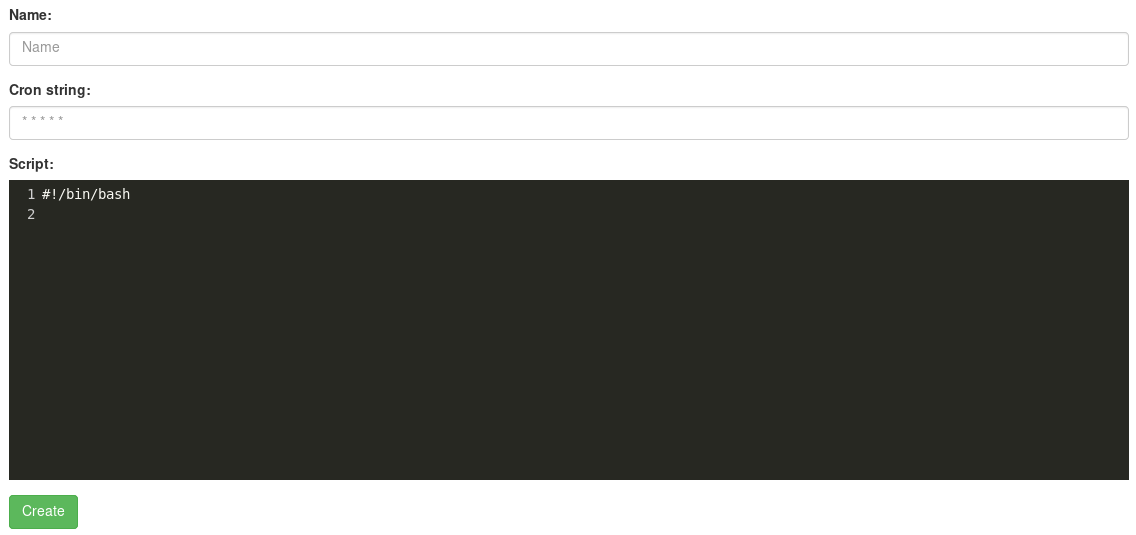
\includegraphics[width=1.00\textwidth]{img/scheduler.png}
  \caption[Scheduler]
  {Scheduler}\label{fig:scheduler}
  \rule[1ex]{\textwidth}{0.25pt}
\end{figure}

Enquanto essa tarefa era desenvolvida, foram explicadas partes da arquitetura e organização da plataforma nas reuniões diárias do \gls{SCRUM}. Também ocorriam momentos nos quais eram ensinados procedimentos de uso do \gls{AWS}, principalmente do \gls{EC2} e \gls{S3}, esses momentos foram de suma importância para a realização de tarefas futuras, pois a \nomeEmpresa~utiliza serviços do \gls{AWS} para a maior parte da aplicação.\\

A segunda grande tarefa realizada foi a implementação do \gls{OAuth2} no \gls{backend} e \gls{frontend}. Em ambos os casos o desenvolvimento foi realizado em conjunto com outro membro mais experiente do time, de forma pareada, afim de promover a familiarização com o código e arquitetura existente.\\

Após esse período de familiarização, começaram a ser atribuídas tarefas da área de \gls{ops}. A primeira se resumiu a usar o \gls{scheduler} para automatizar a geração de relatórios de uso da plataforma, que antes eram gerados de forma manual semanalmente. Foi para o armazenamento dos relatórios, foi utilizado o \gls{S3}.\\

Outra importante tarefa na área de \gls{ops} foi a implementação do \gls{Teste AB}, dividida em duas etapas. Primeiramente houve uma \gls{POC} para entender possíveis ferramentas que poderiam ser usadas. Foi decidido que o \gls{Teste AB} seria implementado diretamente em \gls{PHP} no código da aplicação, permitindo controle de separação por porcentagem de acessos e múltiplas variações para o teste.\\

O código na Listagem~\ref{src:abtest} ilustra a parte principal da implementação, que verifica se a requisição \gls{HTTP} possui um \gls{cookie} de identificação do teste, ou se é necessário gerar um novo baseado nas variações e probabilidades configuradas\\

\begin{lstlisting}[
  language=PHP,
  caption=Teste AB,
  label=src:abtest
]
if ($existing_cookie) {
  return $variations[$existing_cookie]['url'];
} else {
  $random_seed = $this->get_random_seed($settings['seed_method']);
  $variation = $this->select_variation($random_seed, $variations);

  $new_cookie = array(
      'name' => $settings['cookie']['name'],
      'value' => $variation,
      'expire' => $settings['cookie']['expiration'],
      'path' => '/'
      );
  $this->input->set_cookie($new_cookie);
  return $variations[$variation]['url'];
}
\end{lstlisting}

Após a implementação do \gls{Teste AB}, foi iniciada a implantação do sistema de build e testes \gls{Jenkins} para que houvesse a automatização dos testes programáticos e \gls{checkstyle}, assim como geração de imagens \gls{Docker} do projeto. Com objetivo de atingir \gls{CD}\\

O planejamento inicial incluiu apenas a execução de testes e verificação de \gls{checkstyle}, para todas as tecnologias usadas no produto: \gls{PHP}, \gls{Node} e \gls{Vue}. A Figura~\ref{fig:jenkinsBuild} mostra o exemplo de uma build realizada com o \gls{Jenkins}\\

\begin{figure}[h]
  \rule[1ex]{\textwidth}{0.25pt}
  \centering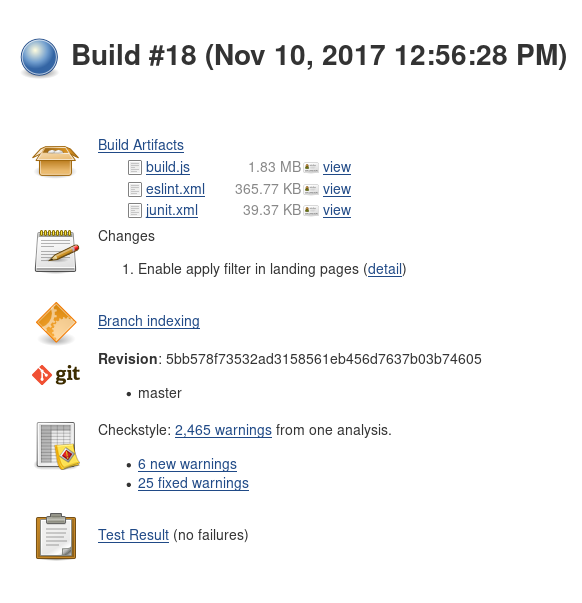
\includegraphics[width=0.70\textwidth]{img/JenkinsBuild.png}
  \caption[Jenkins Build]
  {Jenkins Build}\label{fig:jenkinsBuild}
  \rule[1ex]{\textwidth}{0.25pt}
\end{figure}

Foram realizadas duas tarefas grandes de \gls{backup}, uma do blog da empresa e outra dos dados da base de produção. Em ambos os casos foi escolhido usa o \gls{S3} para armazenamento dos dados copiados, principalmente pelo baixo custo e facilidade de uso.\\


% Descreva quais atividades foram realizadas durante o projeto.
%
% Para cada atividade realizada, discuta também qual foi a dinâmica de trabalho --- por exemplo, se foi utilizada a metodologia SCRUM ou algo similar.
%
% Se apropriado, você apresentar algoritmos ou códigos, como o ilustrado na Listagem~\ref{src:code1}, mas deve explicar o seu funcionamento no texto.

% \begin{lstlisting}[
%   language=C,
%   caption=Exemplo de código,
%   label=src:code1
% ]
% #include <stdio.h>
% int main(){
%   int i=0, j=1;
%   printf("i:%d j:%d\n",i,j);
%   return;
% }
% \end{lstlisting}
%
% Você também pode fazer uso de figuras (como a Figura~\ref{fig:fig1}), mas deve explicar a figura no texto.
%
% \begin{figure}[!ht]
%   \rule[1ex]{\textwidth}{0.25pt}
%   \centering
\includegraphics[width=0.25\textwidth]{img/logoICMC.png}
%   \caption[Exemplo de figura]
%   {Exemplo de figura}\label{fig:fig1}
%   \rule[1ex]{\textwidth}{0.25pt}
% \end{figure}


\section{Problemas resolvidos}

Os principais problemas que foram resolvidos na duração do estágio foram principalmente relacionados a automatização de procedimentos.\\

A implementação do \gls{scheduler} facilitou a realização de muitas tarefas, permitindo o agendamento de atividades recorrentes com facilidade. Com ele foi possível solucionar o problema de geração manual de relatórios toda a semana, permitindo que não fosse necessário executar vários scripts manualmente. Também foi possível, com o \gls{scheduler}, realizar \glspl{backup} diários sem o custo de alocar uma pessoa para essa tarefa.\\

Outra solução importante gerada a partir do trabalho realizado foi a possibilidade de verificar resultados de testes automatizados e \gls{checkstyle} na interface do \gls{Jenkins}. Na Figura~\ref{fig:jenkinsCheckstyle} é possível ver um dos gráficos gerados pelo sistema. No eixo horizontal podemos ver o número da build e no vertical a quantidade de avisos de alta prioridade (em vermelho) e baixa prioridade (em amarelo) de \gls{checkstyle}. É possível notar que houve uma diminuição grande na quantidade de avisos com o tempo.

\begin{figure}[h]
  \rule[1ex]{\textwidth}{0.25pt}
  \centering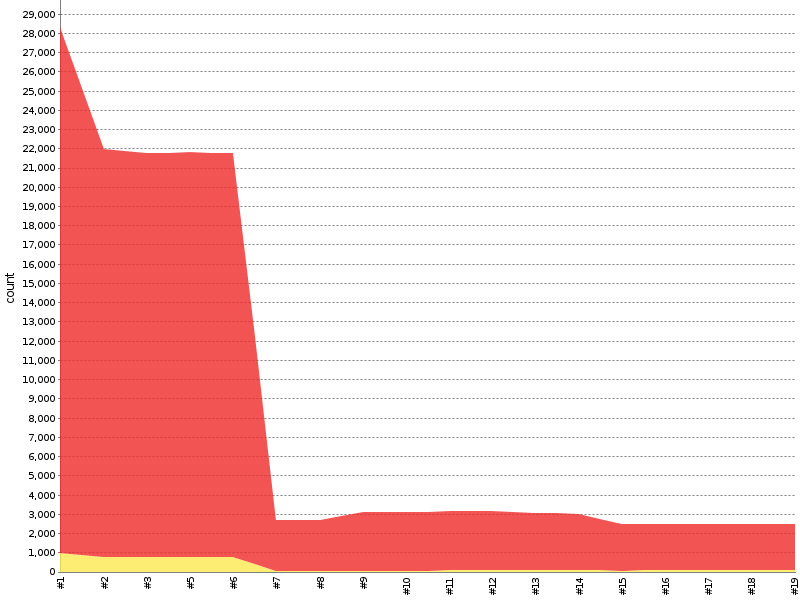
\includegraphics[width=0.70\textwidth]{img/Jenkins.png}
  \caption[Jenkins Checkstyle Trend]
  {Jenkins Checktyle Trend}\label{fig:jenkinsCheckstyle}
  \rule[1ex]{\textwidth}{0.25pt}
\end{figure}

\section{Técnicas, métodos e tecnologias envolvidas}

Durante todo o período do estágio, foi utilizada metodologia de desenvolvimento \gls{SCRUM}. Os primeiros sprints tiveram duração de uma semana em um time com 5 desenvolvedores e um \gls{SCRUM} Master, que ocasionalmente realizava tarefas do sprint. Após um tempo o time decidiu adotar sprints de duas semanas, mas foi retomada a duração inicial após três sprints. Para a organização do time, são utilizadas ferramentas como \href{https://trello.com/}{Trello} para organização de tarefas, \href{https://slack.com/}{Slack} para comunicação dentro do time e \href{https://www.nuclino.com/}{Nuclino} para documentação.\\

Para a infraestrutura, são usados vários serviços da \href{https://aws.amazon.com/}{\gls{AWS}}, como \href{https://aws.amazon.com/ec2/}{\gls{EC2}} para hospedagem dos serviços, \href{https://aws.amazon.com/ecr/}{\gls{ECR}} para hospedagem de imagens \gls{Docker}, \href{https://aws.amazon.com/cloudwatch/}{Cloud Watch} para monitoramento de eventos em produção e \href{https://aws.amazon.com/s3/}{\gls{S3}} para armazenamento de relatórios e backups. Também são usados vários outros serviços não ligados a Amazon, como \href{https://www.hostgator.com.br/}{Hostgator} para hospedagem da plataforma legada e \href{https://www.cloudflare.com/br/}{Cloud Flare} para gerenciamento de \gls{DNS}.\\

As tecnologias envolvidas na plataforma podem ser separadas em três categorias. A primeira são as tecnologias de \gls{frontend}, que incluem \gls{HTML}, \gls{CSS} e \gls{javascript} com \gls{Vue}. No \gls{backend} são usadas as linguagens de programação \gls{PHP} com \href{https://codeigniter.com/}{CodeIgniter} e \href{https://silex.symfony.com/}{Silex} e \gls{javascript} com \gls{Node}. Na terceira categoria se encaixam tecnologias de apoio e infraestrutura, como \href{https://www.docker.com/}{\gls{Docker}} para a execução dos processos em \glspl{container}, \href{https://www.mongodb.com/}{Mongo DB} e \href{https://www.mysql.com/}{MySql} para as bases de dados, \href{https://docs.docker.com/docker-for-aws/}{\gls{Docker} for \gls{AWS}} para a integração com as máquinas da \gls{EC2}, \href{https://traefik.io/}{Træfik} para gerenciamento de trafego nos ambientes de teste e \href{https://analytics.google.com/analytics/}{Google Analytics} para medir métricas da plataforma\\

Para o desenvolvimento de novas funcionalidades, é utilizado o método \gls{TDD}, que visa a criação de testes da aplicação antes de iniciar o desenvolvimento de uma nova funcionalidade. Com testes unitários é possível facilitar o desenvolvimento, por diminuir o tempo de teste.

% Descreva os métodos, técnicas  e tecnologias
% envolvidos  ou que  foram utilizados  para a  condução das  atividades
% durante  o estágio.  Por exemplo:  (i)  no caso  dos métodos,  pode-se
% apresentar XP (eXtreme Programming) e SCRUM, métodos empregados para o
% teste de  sistemas, entre  outros; (ii) No  caso de  técnicas, pode-se
% descrever técnicas da UML, técnicas de teste, entre outros; e (iii) no
% caso  de  tecnologias,  pode-se descrever  ferramentas  (por  exemplo,
% Spring, Hibernate,  Struts, entre  outros), linguagens  de programação
% (por exemplo, Java), padrões de projeto utilizadas, entre outros.
%
% Faça  referências bibliográficas  atuais e  de fontes
% relevantes  (evite  sites,  privilegie   livros  ou  artigos);  mostre
% diferentes  tecnologias e  faça comparações,  quando for  o caso.  Não
% esquecer de citar a fonte corretamente, por exemplo~\cite{MichettiJavaMagazine2013}.

\section{Impacto}

Quais foram as pessoas/entidades afetadas por esses resultados? Quem são  as pessoas/entidades que potencialmente serão afetadas?

Fale sobre a relevância da solução do(s) problema(s) para a empresa e seu(s) cliente(s).

Você deve omitir informações sigilosas.

Discuta também sobre a relevância para sua formação a  participação na solução do(s) problema(s).

\section{Problemas não resolvidos}

Apresente quais os problemas que não puderam ser resolvidos --- e justifique.
